% Options for packages loaded elsewhere
\PassOptionsToPackage{unicode}{hyperref}
\PassOptionsToPackage{hyphens}{url}
%
\documentclass[
]{book}
\usepackage{amsmath,amssymb}
\usepackage{lmodern}
\usepackage{iftex}
\ifPDFTeX
  \usepackage[T1]{fontenc}
  \usepackage[utf8]{inputenc}
  \usepackage{textcomp} % provide euro and other symbols
\else % if luatex or xetex
  \usepackage{unicode-math}
  \defaultfontfeatures{Scale=MatchLowercase}
  \defaultfontfeatures[\rmfamily]{Ligatures=TeX,Scale=1}
\fi
% Use upquote if available, for straight quotes in verbatim environments
\IfFileExists{upquote.sty}{\usepackage{upquote}}{}
\IfFileExists{microtype.sty}{% use microtype if available
  \usepackage[]{microtype}
  \UseMicrotypeSet[protrusion]{basicmath} % disable protrusion for tt fonts
}{}
\makeatletter
\@ifundefined{KOMAClassName}{% if non-KOMA class
  \IfFileExists{parskip.sty}{%
    \usepackage{parskip}
  }{% else
    \setlength{\parindent}{0pt}
    \setlength{\parskip}{6pt plus 2pt minus 1pt}}
}{% if KOMA class
  \KOMAoptions{parskip=half}}
\makeatother
\usepackage{xcolor}
\IfFileExists{xurl.sty}{\usepackage{xurl}}{} % add URL line breaks if available
\IfFileExists{bookmark.sty}{\usepackage{bookmark}}{\usepackage{hyperref}}
\hypersetup{
  pdftitle={BioSci 1540: Computational Biology},
  pdfauthor={Nathan L. Brouwer},
  hidelinks,
  pdfcreator={LaTeX via pandoc}}
\urlstyle{same} % disable monospaced font for URLs
\usepackage{color}
\usepackage{fancyvrb}
\newcommand{\VerbBar}{|}
\newcommand{\VERB}{\Verb[commandchars=\\\{\}]}
\DefineVerbatimEnvironment{Highlighting}{Verbatim}{commandchars=\\\{\}}
% Add ',fontsize=\small' for more characters per line
\usepackage{framed}
\definecolor{shadecolor}{RGB}{248,248,248}
\newenvironment{Shaded}{\begin{snugshade}}{\end{snugshade}}
\newcommand{\AlertTok}[1]{\textcolor[rgb]{0.94,0.16,0.16}{#1}}
\newcommand{\AnnotationTok}[1]{\textcolor[rgb]{0.56,0.35,0.01}{\textbf{\textit{#1}}}}
\newcommand{\AttributeTok}[1]{\textcolor[rgb]{0.77,0.63,0.00}{#1}}
\newcommand{\BaseNTok}[1]{\textcolor[rgb]{0.00,0.00,0.81}{#1}}
\newcommand{\BuiltInTok}[1]{#1}
\newcommand{\CharTok}[1]{\textcolor[rgb]{0.31,0.60,0.02}{#1}}
\newcommand{\CommentTok}[1]{\textcolor[rgb]{0.56,0.35,0.01}{\textit{#1}}}
\newcommand{\CommentVarTok}[1]{\textcolor[rgb]{0.56,0.35,0.01}{\textbf{\textit{#1}}}}
\newcommand{\ConstantTok}[1]{\textcolor[rgb]{0.00,0.00,0.00}{#1}}
\newcommand{\ControlFlowTok}[1]{\textcolor[rgb]{0.13,0.29,0.53}{\textbf{#1}}}
\newcommand{\DataTypeTok}[1]{\textcolor[rgb]{0.13,0.29,0.53}{#1}}
\newcommand{\DecValTok}[1]{\textcolor[rgb]{0.00,0.00,0.81}{#1}}
\newcommand{\DocumentationTok}[1]{\textcolor[rgb]{0.56,0.35,0.01}{\textbf{\textit{#1}}}}
\newcommand{\ErrorTok}[1]{\textcolor[rgb]{0.64,0.00,0.00}{\textbf{#1}}}
\newcommand{\ExtensionTok}[1]{#1}
\newcommand{\FloatTok}[1]{\textcolor[rgb]{0.00,0.00,0.81}{#1}}
\newcommand{\FunctionTok}[1]{\textcolor[rgb]{0.00,0.00,0.00}{#1}}
\newcommand{\ImportTok}[1]{#1}
\newcommand{\InformationTok}[1]{\textcolor[rgb]{0.56,0.35,0.01}{\textbf{\textit{#1}}}}
\newcommand{\KeywordTok}[1]{\textcolor[rgb]{0.13,0.29,0.53}{\textbf{#1}}}
\newcommand{\NormalTok}[1]{#1}
\newcommand{\OperatorTok}[1]{\textcolor[rgb]{0.81,0.36,0.00}{\textbf{#1}}}
\newcommand{\OtherTok}[1]{\textcolor[rgb]{0.56,0.35,0.01}{#1}}
\newcommand{\PreprocessorTok}[1]{\textcolor[rgb]{0.56,0.35,0.01}{\textit{#1}}}
\newcommand{\RegionMarkerTok}[1]{#1}
\newcommand{\SpecialCharTok}[1]{\textcolor[rgb]{0.00,0.00,0.00}{#1}}
\newcommand{\SpecialStringTok}[1]{\textcolor[rgb]{0.31,0.60,0.02}{#1}}
\newcommand{\StringTok}[1]{\textcolor[rgb]{0.31,0.60,0.02}{#1}}
\newcommand{\VariableTok}[1]{\textcolor[rgb]{0.00,0.00,0.00}{#1}}
\newcommand{\VerbatimStringTok}[1]{\textcolor[rgb]{0.31,0.60,0.02}{#1}}
\newcommand{\WarningTok}[1]{\textcolor[rgb]{0.56,0.35,0.01}{\textbf{\textit{#1}}}}
\usepackage{longtable,booktabs,array}
\usepackage{calc} % for calculating minipage widths
% Correct order of tables after \paragraph or \subparagraph
\usepackage{etoolbox}
\makeatletter
\patchcmd\longtable{\par}{\if@noskipsec\mbox{}\fi\par}{}{}
\makeatother
% Allow footnotes in longtable head/foot
\IfFileExists{footnotehyper.sty}{\usepackage{footnotehyper}}{\usepackage{footnote}}
\makesavenoteenv{longtable}
\usepackage{graphicx}
\makeatletter
\def\maxwidth{\ifdim\Gin@nat@width>\linewidth\linewidth\else\Gin@nat@width\fi}
\def\maxheight{\ifdim\Gin@nat@height>\textheight\textheight\else\Gin@nat@height\fi}
\makeatother
% Scale images if necessary, so that they will not overflow the page
% margins by default, and it is still possible to overwrite the defaults
% using explicit options in \includegraphics[width, height, ...]{}
\setkeys{Gin}{width=\maxwidth,height=\maxheight,keepaspectratio}
% Set default figure placement to htbp
\makeatletter
\def\fps@figure{htbp}
\makeatother
\setlength{\emergencystretch}{3em} % prevent overfull lines
\providecommand{\tightlist}{%
  \setlength{\itemsep}{0pt}\setlength{\parskip}{0pt}}
\setcounter{secnumdepth}{5}
\usepackage{booktabs}
\ifLuaTeX
  \usepackage{selnolig}  % disable illegal ligatures
\fi
\usepackage[]{natbib}
\bibliographystyle{apalike}

\title{BioSci 1540: Computational Biology}
\author{Nathan L. Brouwer}
\date{2021-08-13}

\begin{document}
\maketitle

{
\setcounter{tocdepth}{1}
\tableofcontents
}
\hypertarget{welcome}{%
\chapter{Welcome}\label{welcome}}

This is the syllabus.

\begin{Shaded}
\begin{Highlighting}[]
\FunctionTok{install.packages}\NormalTok{(}\StringTok{"bookdown"}\NormalTok{)}
\CommentTok{\# or the development version}
\CommentTok{\# devtools::install\_github("rstudio/bookdown")}
\end{Highlighting}
\end{Shaded}

\hypertarget{course-outline}{%
\chapter{Course outline}\label{course-outline}}

\hypertarget{unit1-1-getting-started}{%
\section{UNIT1 1: Getting started}\label{unit1-1-getting-started}}

\hypertarget{week-1-hello-computational-biology}{%
\subsection{Week 1: Hello Computational Biology!}\label{week-1-hello-computational-biology}}

Reading: NIH Working definition of bioinformatics and computational biology
Supplemental reading: Markowetz (2017). All biology is computational biology
Supplemental reading: Poisot et al (2019). Data based, synthesis drive: Setting the agenda for computational ecology

Supplemental reading: Wikipedia. Computational biology

\hypertarget{week-2-r-camp}{%
\subsection{Week 2: R Camp}\label{week-2-r-camp}}

Reading: Thieme (2018). R generation

\hypertarget{week-3-stats-camp}{%
\subsection{Week 3: Stats Camp}\label{week-3-stats-camp}}

Reading: Meillere et al (2015). Traffic noise exposure affects telomere length in nestling house sparrows

\hypertarget{unti-2-computational-ecology}{%
\section{UNTI 2: Computational Ecology}\label{unti-2-computational-ecology}}

Reading: Dennis et al (1991) Estimation of growth and extinction parameters for endangered species

See Abstract, Introduction and Grizzly bear case study (pg 131-133).
Reference: Morris and Doak (2002). Quantitative conservation biology.
Reference: Steven (2009). A primer of ecology in R.

\hypertarget{unit-3-phylogenetics-bioinformatics}{%
\section{UNIT 3: Phylogenetics \& Bioinformatics}\label{unit-3-phylogenetics-bioinformatics}}

Higgs and Atwood 2005. Bioinformatics and Molecular Evolution
Lycett et al 2007. Phylogenetic analyses of behavior support existence of culture among wild
chimpanzees
Lycett et al 2010. Are behavioral differences among wild chimpanzee communities genetic or
cultural? An assessment using tool‐use data and phylogenetic methods.

\hypertarget{unit-4-bioinformatics-2---sequence-alignment-and-blast-searches}{%
\section{UNIT 4: Bioinformatics 2 - Sequence Alignment and BLAST searches}\label{unit-4-bioinformatics-2---sequence-alignment-and-blast-searches}}

Hildebrand and Soriano (1999). Shroom, a PDZ domain-containing actin-binding protein, is
required for neural tube morphogenesis in mice. Cell. (link ; pdf). See section '' shrm
Encodes a Novel PDZ Domain Protein'' and Figure 4, pg 488-489.
Hagens, Hilderand et al (2006). A new standard nomenclature for proteins related to Apx and
Shroom (link)

\hypertarget{unit-5-bioinformatics-3---algorithms-and-statistics-of-blast}{%
\section{Unit 5: Bioinformatics 3 - Algorithms and statistics of BLAST}\label{unit-5-bioinformatics-3---algorithms-and-statistics-of-blast}}

\hypertarget{intro}{%
\chapter{Introduction}\label{intro}}

This is the syllabus

Your first assignment in the class will be to read through the syllabus and complete a ``Syllabus treasure hunt'' assignment on TopHat. After you've complete that assignment feel free to contact me with any questions you have about course policies.

\hypertarget{meeting-times}{%
\chapter{Meeting times}\label{meeting-times}}

\hypertarget{instructor}{%
\chapter{Instructor}\label{instructor}}

\textbf{Nathan L. Brouwer}, PhD
Office: Crawford Hall\\
A351 (the ``Bridge'')\\
Email: nlb24 at pitt.edu

\hypertarget{academic-integrity}{%
\chapter{Academic integrity}\label{academic-integrity}}

Dr.~Brouwer, the Bio Sci department, and the University all take academic integrity very seriously. Cheating includes any form of plagiarism, including copying other students' work or using other resources without proper attribution.

\begin{enumerate}
\def\labelenumi{\arabic{enumi}.}
\tightlist
\item
  If you are caught cheating on a graded assignment, you will receive a zero on the assignment.
\item
  If you are caught cheating on an exam, you will receive a zero on the exam, an F in the course, and an Academic Integrity Violation Report will be filed.
\end{enumerate}

Below is the University's Policy on Academic Integrity:

\begin{quote}
``Students in this course are expected to comply with the University of Pittsburgh School of Arts \& Sciences Academic Integrity Code located at www.as.pitt.edu/faculty/policy/integrity.html. Any student suspected of failing to meet the student obligations of the code during the semester will be required to participate in the procedures for adjudication, initiated at the instructor level. This may include, but is not limited to, confiscation of the assignment of any individual suspected of violating the code. A minimum sanction of a zero score for the assignment will be imposed. Violation of the Academic Integrity Code requires the instructor to submit an Academic Integrity Violation Report to the Dean.''
\end{quote}

\hypertarget{assessments---homework-policies}{%
\chapter{Assessments - Homework policies}\label{assessments---homework-policies}}

Additional homework will be assigned via TopHat or Canvas. No late assignments will be accepted. Once an assignment closes on TopHat it will no longer be accepted. There will be no makeup homework assignments given. If you miss an assignment it will receive a zero. Your lowest 2 assignment scores will be dropped. This calculation will not be done until after finals.

\hypertarget{assessments}{%
\chapter{Assessments Overview}\label{assessments}}

The primary form of assessment in the course will be regular tests (5).

Other forms of assessment may include,
1. Test revisions (aka Test Reworks), which will count as a form of homework.\\
1. Quiz questions related to lecture videos, code checkpoints to assure that you can execute key functions, and software checkpoints to assure that you have the proper software involved.
1. Additional homework
1. Practice tests

\hypertarget{online-test-taking-policies}{%
\section{Online Test-taking policies}\label{online-test-taking-policies}}

Tests may be administered online.

\hypertarget{final-exam-policies}{%
\section{Final Exam Policies}\label{final-exam-policies}}

The final exam will \ldots{}
1, Take place during finals week on the day scheduled by the University
1. May be online or in person
1. Is required
1. Follow the general format of other tests.

\hypertarget{assessments-1}{%
\section{Assessments}\label{assessments-1}}

As noted previously, your lowest 2 test score will be dropped. Your next lowest test score can be replaced by your final exam, if your final exam score is higher. The final exam can therefore only benefit your score.

\hypertarget{communication---university-email-policy}{%
\chapter{Communication - University email policy}\label{communication---university-email-policy}}

Each student is issued a University e-mail address (username at pitt.edu). This e-mail address may be used by the University for official communication. Students are expected to read e-mail sent to this account on a regular basis. Failure to read and react to University communications in a timely manner does not absolve the student from knowing and complying with the content of the communications.

The University provides an e-mail forwarding service that allows students to read their e-mail via other service providers. Students that choose to forward their e-mail from their pitt.edu address to another address do so at their own risk. If e-mail is lost as a result of forwarding, it does not absolve the student from responding to official communications sent to their University e-mail address.

To forward e-mail sent to your University account, go to \url{http://accounts.pitt.edu}, log into your account, click on Edit Forwarding Addresses, and follow the instructions on the page. Be sure to log out of your account when you have finished.

For the full E-mail Communication Policy, go to bc.pitt.edu/policies/policy/09/09-10-01.html.

\hypertarget{email_and_canvas_msg}{%
\chapter{Course communication - Email and Canvas Messages}\label{email_and_canvas_msg}}

Announcements to the whole course will occur typically on Friday afternoons. Other communcation related to course administration will also occur via Canvas message.

Your can message me on Canvas or email me at nlb24 at pitt.edu.

Please ``Comp Bio'' as the 1st thing in your email subject line with an informative bit of information as the ``\ldots{}''. Eg ``Comp Bio 2: problem accessing TopHat''.

If you use another email service as your primary email (eg GMail) please set your Pitt email to forward there.

For info on forwarding your Pitt email to your personal account follow this link: \url{https://bit.ly/2Riz7dx}

I try to answer all emails received on weekdays before 5 pm within 24-36 hrs. Emails recieved after 5 pm will be answered at the earliest the following morning. Emails received on the weekend will be answered Monday.

Please consult this syllabus before asking questions about course policies and the schedule, and refer to relevant information such as URLs, subject headings or dates. Screengrabs are super helpful. If the entire answer to your question can be found in the syllabus I will likely respond by saying ``This is in the syllabus, Cheers, Dr.~B.''*.

Questions relevant to the whole class may be reposted (with identifying details removed).

\hypertarget{course-communication---overview}{%
\chapter{Course communication - Overview}\label{course-communication---overview}}

\hypertarget{primary-modes-of-communication}{%
\section{Primary modes of communication}\label{primary-modes-of-communication}}

All important details will be sent via Canavas message and mentioned/discussed in class. It is your responsiblity to regularly check Canvas messages to stay abreast of the course.

\hypertarget{secondary-modes-of-communication}{%
\section{Secondary modes of communication}\label{secondary-modes-of-communication}}

\hypertarget{github-issues}{%
\subsection{Github ``issues''}\label{github-issues}}

In this class we will be making extensive use of the code management site GitHub. Most communcation about homework and other assignments will occur via GitHubs Issues feature. Moreover, to foster discussion we will use GitHub issues to create forums around assignments and you will be required to submit comments.

\hypertarget{microsoft-share-point}{%
\subsection{Microsoft Share Point}\label{microsoft-share-point}}

Files containing code for this course will be distributed using MicroSoft Sharepoint. Sharepoint has messaging features which I may experitment but will not rely on.

\hypertarget{catalog-description}{%
\chapter{Catalog description}\label{catalog-description}}

\begin{quote}
``This course is designed to give students a broad understanding of how computational approaches can be used to solve problems in biology. Both the biological and computational underpinnings of the methods will be addressed.''
\end{quote}

\hypertarget{course-materials-overview}{%
\chapter{Course materials overview}\label{course-materials-overview}}

Thanks to an Open Educational Resources (OER) grant from The Office of the Provost, there are no books to buy for this course - all course materials are free and will be provided digitally through Canvas.

Reading will take many forms: files containing computer code (scripts), articles and blog posts, as well as textbook. However, we'll be taking a very novel approach to the textbook for this course: \textbf{you will actually be building it yourself!}

Details will be provided in-class, but the gist regarding the textbook is:
1. Most weeks you will be provided 1 or 2 chapters of the book in the form of computer files (``scripts'').
1. For homework you will do exercises embedded in the chapters.
1. When the exercises are successfully completed you will be able to convert the files to Web Pages and post them to your own Portofolio of book chapters and other completed activites.

\hypertarget{course-materials---software}{%
\chapter{Course materials - Software}\label{course-materials---software}}

Installation and account creation for all software will be covered in detail during class or via assignmetns and accompanying videos. If you want to get prepared early for the course you can explore these on your own.

\hypertarget{primary-software}{%
\section{Primary software}\label{primary-software}}

\hypertarget{programming-environment-r}{%
\subsection{Programming environment: R}\label{programming-environment-r}}

We will use the open-source language R for almost everything in this course.

\textbf{NOTE}: If you have used R before that's awesome! \textbf{Please update your installation when the class begins} - R goes through regular updates and works best with the newest version.

If you are having trouble installing R an excellent resource is:
\url{https://learningstatisticswithr.com/book/introR.html}

R Core Team (2021). R: A language and environment for statistical computing. R Foundation for Statistical Computing, Vienna, Austria. www.R-project.org/.

\hypertarget{integrated-developement-environment}{%
\subsection{Integrated developement environment}\label{integrated-developement-environment}}

We'll use RStudio as the front-end for working with R.

\textbf{NOTE}: If you've use RStudio before please update it when the course begins.

\textbf{RStudio:} www.rstudio.com/products/rstudio/download/\#download

\hypertarget{cloud-based-r}{%
\subsection{Cloud-based R}\label{cloud-based-r}}

As a back-up to running R on your desktop I'll also introduce you to RStudio Cloud. There are also several excellent \href{https://rstudio.cloud/learn/primers}{primers} which we'll use.

\textbf{RStudio cloud:} \url{https://rstudio.cloud/}

\hypertarget{code-sharing}{%
\section{Code sharing}\label{code-sharing}}

\hypertarget{microsoft-sharepoint}{%
\subsection{Microsoft SharePoint}\label{microsoft-sharepoint}}

R code and other files will be distributed to you via a personal folder on SharePoint, accessed via your OneDrive account.

You will need to ``sync'' your OneDrive account to your computer desktops to allow me to help you with your work. No code files will be shared via email or Canvas during the course.

\textbf{NOTE}: If you do not have access to a computer you can sync your OneDrive account please contact me so we can workout a system.

\hypertarget{github}{%
\subsection{GitHub}\label{github}}

Most code for this course will be available on GitHub and you will need to create an account for some activities.

\textbf{GitHub:} \url{https://github.com/}

\hypertarget{r-packages}{%
\section{R packages}\label{r-packages}}

Many R packages (aka libraries) will be used in this course. Below are several key ones.

\hypertarget{swirl}{%
\subsection{swirl}\label{swirl}}

\emph{swirl} is an R package that sets up interactive tutorials in your R console. It works both on desktop computers and RStudio cloud and is an excellent tool for learning and reviewing R.

\hypertarget{bioconductor}{%
\subsection{Bioconductor}\label{bioconductor}}

\textbf{Bioconductor} is a clearing house and repository for high-grade bioinformatics and computational biology software using R.

\hypertarget{bibliography}{%
\chapter{Bibliography}\label{bibliography}}

Below are resources that you may wish to use for reference during the course or in the future for review.

\hypertarget{bioinformatics-computational-biology}{%
\section{Bioinformatics \& computational biology}\label{bioinformatics-computational-biology}}

\textbf{Pevsner 2015. Bioinformatics and functional genomics. 3rd edition.}\\
Available \textbf{FREE} via the Pitt library, though you can only download a few chapters at a time. I do \textbf{NOT} recommend buying a hard copy because I am currently only planning on using the first 1/3 of the book. If you want a hard copy and buy it used be sure to get the 3rd edition.

\hypertarget{phylogenetics}{%
\section{Phylogenetics}\label{phylogenetics}}

\textbf{Wiley, EO and BS Liberman. 2011. Phylogenetics: Theory and Practice of Phylogenetic Systematics. 2nd ed.}\\
Available \textbf{FREE} via the Pitt library, though you can only download a few chapters at a time. I do \textbf{NOT} recommend buying a hard copy because I am currently only planning on using a few chapters. If you want a hard copy and buy it used be sure to get the 2nd edition.

Focal chapters in Wiley and Liberman (2011):
* Chapter 4: Tree graphs
* Chapter 5: Characters \& homology
* Chapter 6: Parsimony \& parsimony analysis
* Chapter 7: Parametric phylogenetics

\hypertarget{statistics}{%
\section{Statistics}\label{statistics}}

\textbf{Navarro, D. 2019. Learning Statistics with R}
PDF: \url{https://learningstatisticswithr.com/lsr-0.6.pdf}\\
HTML: \url{https://learningstatisticswithr.com/book/}

Focal chapters in Navarro:
* \href{https://learningstatisticswithr.com/book/introR.html}{``Getting started with R''}
* \href{https://learningstatisticswithr.com/book/mechanics.html}{``Additional R concepts''}
* \href{https://learningstatisticswithr.com/book/descriptives.html}{``Descriptive statistics''}
* \href{https://learningstatisticswithr.com/book/datahandling.html}{``Pragmatic matters''}
* \href{https://learningstatisticswithr.com/book/graphics.html\#hist}{``Drawing graphs''}
* \href{https://learningstatisticswithr.com/book/scripting.html}{``Basic programming''}
* \href{https://learningstatisticswithr.com/book/probability.html}{``Introduction to probability''}

\hypertarget{reference-books}{%
\section{Reference Books}\label{reference-books}}

Cadotte \& Davies. Phylogenies in ecology: A guide to concepts and methods.
Free from library. Covers the use of phylogenies in community ecology and trait evolution.

Nei and Kumar. Molecular evolution and phylogenetics.
Free from library. Contains more mathematical treatments of maximum likelihood etc.

\hypertarget{reference-articles-blogs-etc}{%
\section{Reference articles, blogs etc}\label{reference-articles-blogs-etc}}

Altman. 2009. \href{https://rbaltman.wordpress.com/2009/02/18/bioinformatics-computational-biology-same-no/}{Bioinformatics \& computational biology = Same? No.} ttps://rbaltman.wordpress.com

Gregory 2008. Understanding evolutionary trees. Evo Edu Outreach 1:121-137.

Koonin. 2001. Computational genomics. Current Biology 11:R155-R158.

Loman and Watson. 2013. So you want to be a computational biologist? Nature Biotech.

Markowetz, F. 2017. All biology is computational biology. PLoS Biology.

Nascimente, FF et al.~2017. A biologist's guide to Bayesian phylogenetic analysis. Nature Ecology \& Evolution. See GitHub repo and blog posts.

Nussinov et al.~2015. From ``What is?'' to ``What isn't?'' computational biology. PLoS Computational Biology.

Visser et al 2015. Speeding up ecological and evolutionary computations in R: Essential of high performanc computing for biologists. PLoS Computational Biology.

\hypertarget{DRS}{%
\chapter{Disability Resource \& Services}\label{DRS}}

216 William Pitt Union\\
(412) 648-7890\\
(412) 383-7355 (TYY)

If you have a disability for which you are or may be requesting an accommodation, you are encouraged to contact both your instructor and Disabilities Resources and Services. DRS will verify your disability and determine reasonable accommodations.

\hypertarget{extracredit}{%
\chapter{Extra credit policies}\label{extracredit}}

No extra credit will be offered in this course.

``Buffer questions'' on the mini-tests, test revision, and the final are NOT extra credit.

\hypertarget{file_names}{%
\chapter{File names for homework}\label{file_names}}

All files your create which get submitted for homework need to be in lower case and \textbf{strictly} adhere to this format:

\begin{quote}
``pittemail\_lastname\_assignmenttitle''
\end{quote}

For example:

``nlb24\_brouwer\_assign\_1.rmd''

\hypertarget{course-goals}{%
\section{Course Goals}\label{course-goals}}

The goals of Computational Biology is to introduce you to key concepts relatd to how computers are used to solve biological problems, and build skills essential to your success working on projects related to computational biology and bioinformatics.

\hypertarget{grading-scale}{%
\chapter{Grading scale}\label{grading-scale}}

\textbf{Note}: Students planning to major in Biological Sciences must pass this course with a C (not C- !) or better. Rounding is not done until final grades are computed and is done by computer to 1 decimal place.

Final letter grades are assigned after rounding and is done automatically by Canvas including the decimal value. For example, a score of 91.99\% rounds to 92.0\% and is an A, but a score of 91.94\% rounds to 91.9\% and is an A-.

Note: Students planning to major in Computational Biology must pass this course with a C (not C- !) or better.

\hypertarget{meeting-times-1}{%
\chapter{Meeting times}\label{meeting-times-1}}

The course will meeting in person on Tuesdays and Thursday. There is no recitation for this course.

TopHat will be used during lectures but any questions can be answered outside of class.

Location: 1502 Posvar Hall\\
Daays: Tuesday \& Thursday\\
Times: 4:00PM - 5:15AM

\hypertarget{metnal-health-wellness}{%
\chapter{Metnal health \& wellness}\label{metnal-health-wellness}}

School is hard - please take care of yourself as best you can given the many demands on your time. Diminished mental health, including significant stress, mood changes, excessive anxiety, or problems with sleeping can interfere with your academic performance. You have a support network here at Pitt to help you through challenging times. Acknowledging that you need help, and getting that help, is smart and courageous.

\begin{itemize}
\tightlist
\item
  If you are in an EMERGENCY situation, call 911 or Pitt Police at 412-624-2121.
\item
  If your symptoms are due to FINANCIAL strain, please visit pitt.libguides.com/assistanceresources to see all available University resources.
\item
  If your symptoms are due to strained RELATIONSHIPS, families, or personal crises, please visit the University Counseling Center at www.studentaffairs.pitt.edu/cc/ for free confidential services.
\item
  If your symptoms are strictly related to your COURSE WORK and performance in this course, please contact me.
\end{itemize}

\hypertarget{resources}{%
\section{Resources:}\label{resources}}

\textbf{University Counseling Center}: 412-648-7930\\
\textbf{Sexual Assault Response}: 412-648-7856\\
\textbf{RE:SOLVE crisis network}: 888-796-8226\\
\textbf{Pitt Police}: 412-624-2121\\
\href{https://www.studentaffairs.pitt.edu/pittserves/the-pitt-pantry/}{\textbf{Pitt Pantry food bank}}: \url{https://www.studentaffairs.pitt.edu/pittserves/the-pitt-pantry/}

\hypertarget{office-hours}{%
\chapter{Office hours}\label{office-hours}}

\hypertarget{instructor-office-hours}{%
\section{INSTRUCTOR OFFICE HOURS}\label{instructor-office-hours}}

\hypertarget{uta-office-hours}{%
\section{UTA OFFICE HOURS}\label{uta-office-hours}}

\hypertarget{points}{%
\chapter{Point breakdown}\label{points}}

\hypertarget{semester-schedule}{%
\chapter{Semester schedule}\label{semester-schedule}}

\hypertarget{skills}{%
\chapter{Skills}\label{skills}}

\textbf{Key Skills}:
1. Understanding R code\\
2. Data visualization\\
3. Graph interpretation\\
4. \ldots{}

Key to Computational Biology will be developing skills as a critical practioner and consumer of science. The course will heavily emphasize the application of skills related to scientific programming, including understanding and modifying R code, plotting data, organizing computational workflows, annotating computational projects. A central set of skill we be learnign to intepret the types of graphs used in computational biology, including alignments, phylogenies, networks, heatmaps, and ordination plots. The course will also introduce basic skills related to statistics, probablity, and mathematical modeling. We will also emphasize critical reading and interpretation of the primary literature.

\begin{Shaded}
\begin{Highlighting}[]
\FunctionTok{library}\NormalTok{(ape)}

\FunctionTok{cat}\NormalTok{(}\StringTok{"(((Strix\_aluco:4.2,Asio\_otus:4.2):3.1,"}\NormalTok{,}
\StringTok{"Athene\_noctua:7.3):6.3,Tyto\_alba:13.5);"}\NormalTok{,}
\AttributeTok{file =} \StringTok{"ex.tre"}\NormalTok{, }\AttributeTok{sep =} \StringTok{"}\SpecialCharTok{\textbackslash{}n}\StringTok{"}\NormalTok{)}
\NormalTok{tree.owls }\OtherTok{\textless{}{-}} \FunctionTok{read.tree}\NormalTok{(}\StringTok{"ex.tre"}\NormalTok{)}
\FunctionTok{plot}\NormalTok{(tree.owls)}
\end{Highlighting}
\end{Shaded}

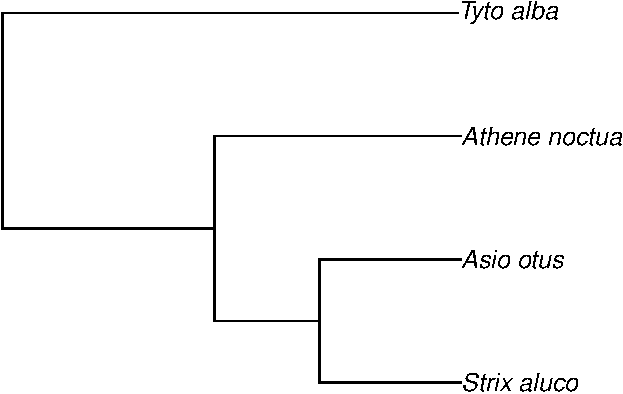
\includegraphics{1540_syllabus_files/figure-latex/unnamed-chunk-2-1.pdf}

\begin{Shaded}
\begin{Highlighting}[]
\FunctionTok{unlink}\NormalTok{(}\StringTok{"ex.tre"}\NormalTok{) }\CommentTok{\# delete the file "ex.tre"}
\end{Highlighting}
\end{Shaded}

\hypertarget{tophat}{%
\chapter{TopHat}\label{tophat}}

\hypertarget{in-class-response-homework-system}{%
\section{In-class response / Homework system}\label{in-class-response-homework-system}}

We will use TopHat in-class and for homework. Please bring a charged TopHat compatible device to all lectures and recitations. See the \textbf{Course Policies} section for information related to if you are not able to answer TopHat questions during class due to technical difficulties.

\href{www.tophat.com}{\textbf{TopHat}}\\
Join Code: \textbf{209015}\\
www.tophat.com

When logging into TopHat it will ask you for your university. Typing in ``University of Pittsburgh'' brings up 3 options: \textbf{select the first one} that just says ``University of Pittsburgh.

\hypertarget{updates-to-schedule-syllabus}{%
\chapter{Updates to schedule \& syllabus}\label{updates-to-schedule-syllabus}}

I reserve the right to update the syllabus, schedule, point allocation and all other components of the course as necessary. If changes occur after the first day of class, they will be clearly communicated in class and via email, and a revised syllabus and schedule distributed. After reading the syllabus and completing the ``Syllabus treasure hunt'' assignment (which will be posted on the first day of class) feel free to contact me with any questions about course policies.

\hypertarget{appendix-graduate-school}{%
\chapter{Appendix: graduate school}\label{appendix-graduate-school}}

If you are considering graduate school you may wish to check out these resource:

So you want to go to graduate school?
O'Connel, Tim. ``A conversation about grad school'' \url{https://eatmorecookies.wordpress.com/2018/07/17/a-conversation-about-grad-school/}

Carson, W.P. 1999. A primer on how to apply and get admitted to graduate school in ecology and evolutionary biology. Bulletin of the Ecological Society of America 80(4):246-250. (PDF here: \url{https://sites.google.com/site/walterpagecarson/publications})

Stearns, S. Some modest advices for graduate students
Bulletin of the Ecological Society of America, 1987 - JSTOR
\url{https://stearnslab.yale.edu/some-modest-advice-graduate-students}

Thoughts on Stearns and Huey
Fox, J. 2015. Re-reading Stearns and Hueys some modest advice to gradate students.
\url{https://dynamicecology.wordpress.com/2015/09/08/rereading-stearns-and-hueys-some-modest-advice-to-graduate-students/}

On the publishing process: a tweet by \citet{dsquintana}
\url{https://twitter.com/dsquintana/status/1154820610750595072?s=20}

\hypertarget{cheat-sheets}{%
\chapter{Cheat sheets}\label{cheat-sheets}}

RStudio produces a number of \href{https://www.rstudio.com/resources/cheatsheets/\#ide}{cheatsheets}; the most useful ones for beginners are below.

Basic R code
\url{http://github.com/rstudio/cheatsheets/raw/master/base-r.pdf}

RStudio
\url{https://github.com/rstudio/cheatsheets/raw/master/rstudio-ide.pdf}

RMarkdown
\url{https://github.com/rstudio/cheatsheets/raw/master/rmarkdown-2.0.pdf}
\url{https://www.rstudio.com/wp-content/uploads/2015/03/rmarkdown-reference.pdf}

Translations of some of these cheat sheets can be found at the bottom of the RStudio page.

\hypertarget{appendix-getting-involved-in-computational-research}{%
\chapter{Appendix: Getting involved in (computational) research}\label{appendix-getting-involved-in-computational-research}}

Approaching a PI - A guide for undergraduates \url{https://thefemalescientist.com/guide/madeleine-hann/2053/approaching-a-pi-a-guide-for-undergraduates-in-stem/}

\hypertarget{shortcuts-in-r}{%
\chapter{Shortcuts in R}\label{shortcuts-in-r}}

Programmers are often obsessed with using keyboard shortcuts. You'll see me use some, and you might want to learn them.

The back of this cheatsheet is a 1-page summary of shortcuts
\url{https://github.com/rstudio/cheatsheets/raw/master/rstudio-ide.pdf}

Another summary sheet of Shortcuts in RStudio is here:
\url{https://support.rstudio.com/hc/en-us/articles/200711853-Keyboard-Shortcuts}

A great blog post on shortcuts is here
\url{https://appsilon.com/r-studio-shortcuts-and-tips/}

\end{document}
